\documentclass[11pt,letterpaper]{article}

% ============================================================================
% PACKAGES
% ============================================================================
\usepackage[utf8]{inputenc}
\usepackage[T1]{fontenc}
\usepackage{helvet}
\renewcommand{\familydefault}{\sfdefault}
\usepackage[margin=0.85in, headheight=28pt]{geometry}
\usepackage{graphicx}
\usepackage{xcolor}
\usepackage{tikz}
\usepackage{tcolorbox}
\usepackage{booktabs}
\usepackage{enumitem}
\usepackage{hyperref}
\usepackage{fancyhdr}
\usepackage{titlesec}
\usepackage{multicol}
\usepackage{listings}
\usepackage{upquote}
\usepackage{amsmath,amssymb}
\usepackage{pgfplots}
\usepackage{array}
\usepackage{longtable}

% Ragged-right paragraph columns to prevent word spacing issues
\newcolumntype{L}[1]{>{\raggedright\arraybackslash}p{#1}}

% Increase vertical spacing between table rows for readability
\renewcommand{\arraystretch}{1.4}

\usepackage{colortbl}
\usepackage{pifont}
\usepackage{setspace}
\usepackage{parskip}
\usepackage{caption}

\pgfplotsset{compat=1.18}
\usetikzlibrary{shapes.geometric, arrows.meta, positioning, calc, decorations.pathreplacing, backgrounds, fit, shadows.blur, matrix, patterns, fadings, shadings}

% ============================================================================
% COLOR DEFINITIONS - Virtual Character Theme (Teal/Purple/Pink)
% ============================================================================
\definecolor{vcdark}{HTML}{1A1A2E}           % Deep navy-purple
\definecolor{vcprimary}{HTML}{16213E}        % Dark blue
\definecolor{vcteal}{HTML}{0F969C}           % Primary teal
\definecolor{vclightteal}{HTML}{6BC6C6}      % Light teal
\definecolor{vcpurple}{HTML}{7B2CBF}         % Accent purple
\definecolor{vcpink}{HTML}{E056FD}           % Bright pink
\definecolor{vcgold}{HTML}{F4D35E}           % Gold accent
\definecolor{successgreen}{HTML}{2ECC71}     % Success green
\definecolor{warningamber}{HTML}{F39C12}     % Warning amber
\definecolor{dangerred}{HTML}{E74C3C}        % Danger red
\definecolor{infoteal}{HTML}{17A2B8}         % Info teal
\definecolor{coolgray}{HTML}{6C757D}         % Cool gray
\definecolor{lightgray}{HTML}{F8F9FA}        % Light background
\definecolor{codebg}{HTML}{F7F7F7}           % Light code background
\definecolor{codetext}{HTML}{333333}         % Dark code text
\definecolor{codekeyword}{HTML}{7B2CBF}      % Purple keywords
\definecolor{codestring}{HTML}{0F969C}       % Teal strings
\definecolor{codecomment}{HTML}{808080}      % Gray comments
\definecolor{codeborder}{HTML}{E0E0E0}       % Border color

% ============================================================================
% HYPERREF SETUP
% ============================================================================
\hypersetup{
  colorlinks=true,
  linkcolor=vcteal,
  urlcolor=vcpurple,
  pdftitle={Virtual Character System - Dual-Speed Cognitive Architecture},
  pdfauthor={AI Agent Team}
}

% ============================================================================
% SPACING AND TYPOGRAPHY
% ============================================================================
\setstretch{1.15}
\setlength{\parskip}{0.5em}
\setlist{nosep, leftmargin=1.5em, itemsep=0.3em}

% ============================================================================
% PAGE STYLE
% ============================================================================
\pagestyle{fancy}
\fancyhf{}
\fancyhead[L]{%
  \begin{tikzpicture}[baseline=-0.5ex]
    \fill[vcteal] (0,0) circle (0.15);
    \fill[vcpurple] (0.35,0) circle (0.1);
    \fill[vcpink] (0.6,0) circle (0.06);
  \end{tikzpicture}
  \hspace{0.3em}\textcolor{vcprimary}{\textsf{\textbf{Virtual Character}}}%
}
\fancyhead[R]{\textcolor{coolgray}{\textsf{\thepage}}}
\fancyfoot[C]{\textcolor{coolgray}{\small\textsf{Dual-Speed Cognitive Architecture Guide}}}
\renewcommand{\headrulewidth}{0pt}
\renewcommand{\footrulewidth}{0pt}

\fancyheadoffset{0pt}
\setlength{\headheight}{32pt}

% ============================================================================
% SECTION FORMATTING
% ============================================================================
\titleformat{\section}
  {\normalfont\LARGE\bfseries\color{vcprimary}}
  {\colorbox{vcteal}{\textcolor{white}{\thesection}}}{0.8em}{}
\titleformat{\subsection}
  {\normalfont\Large\bfseries\color{vcprimary!80}}
  {\thesubsection}{0.6em}{}
\titleformat{\subsubsection}
  {\normalfont\large\color{coolgray}\bfseries}
  {\thesubsubsection}{0.5em}{}

\titlespacing*{\section}{0pt}{3ex plus 1ex minus .2ex}{2ex plus .2ex}
\titlespacing*{\subsection}{0pt}{2.5ex plus 1ex minus .2ex}{1.5ex plus .2ex}

% ============================================================================
% TOC STYLING
% ============================================================================
\setcounter{tocdepth}{2}

% ============================================================================
% TCOLORBOX ENVIRONMENTS
% ============================================================================
\tcbuselibrary{skins,breakable,hooks}

% Key Concept Box
\newtcolorbox{keybox}[1][Key Concept]{
  enhanced,
  breakable,
  colback=vcteal!5,
  colframe=vcteal,
  colbacktitle=vcteal,
  coltitle=white,
  fonttitle=\bfseries\sffamily,
  title={\faBrain\hspace{0.5em}#1},
  boxrule=0pt,
  leftrule=4pt,
  arc=0pt,
  outer arc=0pt,
  left=12pt, right=12pt, top=8pt, bottom=8pt,
  shadow={2pt}{-2pt}{0pt}{black!20}
}

% Warning Box
\newtcolorbox{warnbox}[1][Warning]{
  enhanced,
  breakable,
  colback=dangerred!5,
  colframe=dangerred,
  colbacktitle=dangerred,
  coltitle=white,
  fonttitle=\bfseries\sffamily,
  title={\faExclamationTriangle\hspace{0.5em}#1},
  boxrule=0pt,
  leftrule=4pt,
  arc=0pt,
  outer arc=0pt,
  left=12pt, right=12pt, top=8pt, bottom=8pt,
  shadow={2pt}{-2pt}{0pt}{black!15}
}

% Success/Tip Box
\newtcolorbox{tipbox}[1][Pro Tip]{
  enhanced,
  breakable,
  colback=successgreen!8,
  colframe=successgreen,
  colbacktitle=successgreen,
  coltitle=white,
  fonttitle=\bfseries\sffamily,
  title={\faCheckCircle\hspace{0.5em}#1},
  boxrule=0pt,
  leftrule=4pt,
  arc=0pt,
  outer arc=0pt,
  left=12pt, right=12pt, top=8pt, bottom=8pt,
  shadow={2pt}{-2pt}{0pt}{black!15}
}

% System Box - Purple accent
\newtcolorbox{systembox}[1][System Component]{
  enhanced,
  breakable,
  colback=vcpurple!5,
  colframe=vcpurple,
  colbacktitle=vcpurple,
  coltitle=white,
  fonttitle=\bfseries\sffamily,
  title={\faCog\hspace{0.5em}#1},
  boxrule=0pt,
  leftrule=4pt,
  arc=0pt,
  outer arc=0pt,
  left=12pt, right=12pt, top=8pt, bottom=8pt,
  shadow={2pt}{-2pt}{0pt}{black!15}
}

% Info Box
\newtcolorbox{infobox}[1][Note]{
  enhanced,
  breakable,
  colback=infoteal!5,
  colframe=infoteal,
  colbacktitle=infoteal,
  coltitle=white,
  fonttitle=\bfseries\sffamily,
  title={\faInfoCircle\hspace{0.5em}#1},
  boxrule=0pt,
  leftrule=4pt,
  arc=0pt,
  outer arc=0pt,
  left=12pt, right=12pt, top=8pt, bottom=8pt,
  shadow={2pt}{-2pt}{0pt}{black!15}
}

% TL;DR Summary Box
\newtcolorbox{tldrbox}{
  enhanced,
  breakable,
  colback=vcprimary!3,
  colframe=vcprimary,
  boxrule=1.5pt,
  arc=8pt,
  outer arc=8pt,
  left=15pt, right=15pt, top=12pt, bottom=12pt,
  fontupper=\small,
  before upper={\textcolor{vcteal}{\faRocket}\hspace{0.5em}\textbf{TL;DR}\hspace{0.8em}},
  shadow={3pt}{-3pt}{0pt}{black!20}
}

% ============================================================================
% CODE LISTING STYLE
% ============================================================================
\lstdefinestyle{moderncode}{
  basicstyle=\ttfamily\small\color{codetext},
  keywordstyle=\color{codekeyword}\bfseries,
  stringstyle=\color{codestring},
  commentstyle=\color{codecomment}\itshape,
  backgroundcolor=\color{codebg},
  frame=single,
  rulecolor=\color{codeborder},
  framesep=8pt,
  numbers=left,
  numberstyle=\tiny\color{coolgray},
  numbersep=12pt,
  breaklines=true,
  showstringspaces=false,
  tabsize=4,
  xleftmargin=25pt,
  framexleftmargin=20pt,
  aboveskip=1em,
  belowskip=1em,
  literate={`}{\`}1
}
\lstdefinelanguage{Rust}{
  morekeywords={async,await,fn,pub,struct,impl,enum,match,let,mut,self,Self,use,mod,crate,super,trait,where,for,in,if,else,return,true,false,Some,None,Ok,Err,Result,Option,Vec,String,HashMap,Arc,RwLock,Box,dyn},
  sensitive=true,
  morecomment=[l]{//},
  morecomment=[s]{/*}{*/},
  morestring=[b]",
}
\lstset{style=moderncode, language=Rust}

% ============================================================================
% ICON COMMANDS (pifont replacements)
% ============================================================================
\newcommand{\faRobot}{\ding{70}}
\newcommand{\faCheck}{\ding{51}}
\newcommand{\faCheckCircle}{\ding{51}}
\newcommand{\faTimes}{\ding{55}}
\newcommand{\faTimesCircle}{\ding{55}}
\newcommand{\faExclamationTriangle}{\ding{74}}
\newcommand{\faExclamationCircle}{\ding{74}}
\newcommand{\faLightbulb}{\ding{72}}
\newcommand{\faInfoCircle}{\ding{73}}
\newcommand{\faRocket}{\ding{228}}
\newcommand{\faDatabase}{\ding{115}}
\newcommand{\faTachometerAlt}{\ding{99}}
\newcommand{\faCloud}{\ding{110}}
\newcommand{\faBrain}{\ding{70}}
\newcommand{\faServer}{\ding{115}}
\newcommand{\faProjectDiagram}{\ding{118}}
\newcommand{\faLayerGroup}{\ding{115}}
\newcommand{\faCode}{\texttt{</>}}
\newcommand{\faCog}{\ding{70}}
\newcommand{\faCogs}{\ding{70}}
\newcommand{\faShieldAlt}{\ding{110}}
\newcommand{\faKey}{\ding{70}}
\newcommand{\faEye}{\ding{70}}
\newcommand{\faCloudUploadAlt}{\ding{110}}
\newcommand{\faChartLine}{\ding{70}}
\newcommand{\faBook}{\ding{70}}
\newcommand{\faFileCode}{\ding{70}}
\newcommand{\faListAlt}{\ding{70}}
\newcommand{\faClock}{\ding{70}}
\newcommand{\faSearch}{\ding{70}}
\newcommand{\faVolumeUp}{\ding{70}}
\newcommand{\faUser}{\ding{70}}
\newcommand{\faHeart}{\ding{70}}
\newcommand{\faBolt}{\ding{70}}
\newcommand{\faSync}{\ding{70}}
\newcommand{\faMicrophone}{\ding{70}}

% ============================================================================
% PART PAGE STYLING (simplified - no TikZ overlay for reliability)
% ============================================================================
\newcommand{\partpage}[4]{%
  \clearpage
  \thispagestyle{empty}

  % Header box with gradient simulation
  \noindent\colorbox{vcdark}{%
    \parbox{\dimexpr\textwidth-2\fboxsep}{%
      \vspace{1.5cm}
      \begin{center}
        {\color{white}\large\sffamily PART}\\[0.3cm]
        {\color{vcteal}\fontsize{60}{60}\selectfont\bfseries #1}\\[0.5cm]
        {\color{white}\LARGE\bfseries\sffamily #2}\\[0.3cm]
        {\color{vcteal}\rule{8cm}{2pt}}
      \end{center}
      \vspace{1cm}
    }%
  }

  \vspace{1.5cm}

  % Overview content
  \begin{center}
  \begin{minipage}{0.88\textwidth}
    \begin{tcolorbox}[
      enhanced,
      colback=white,
      colframe=vcteal!50,
      boxrule=1pt,
      arc=6pt,
      left=15pt, right=15pt, top=12pt, bottom=12pt,
      shadow={2pt}{-2pt}{0pt}{black!15}
    ]
    \textcolor{vcprimary}{\faListAlt\hspace{0.5em}\textbf{What's Covered}}
    \vspace{0.5em}

    #3
    \end{tcolorbox}

    \vspace{1em}

    % Icon row
    \begin{center}
    #4
    \end{center}
  \end{minipage}
  \end{center}
}

% ============================================================================
% DOCUMENT
% ============================================================================
\begin{document}

% ============================================================================
% TITLE PAGE
% ============================================================================
\begin{titlepage}

\begin{tikzpicture}[remember picture, overlay]
  % Left panel gradient (full height)
  \shade[left color=vcdark, right color=vcprimary!90]
    (current page.north west) rectangle ([xshift=7cm]current page.south west);

  % Decorative circles on left panel
  \fill[vcteal, opacity=0.15] ([xshift=3.5cm, yshift=-4cm]current page.north west) circle (1.2cm);
  \fill[vcpurple, opacity=0.10] ([xshift=3.5cm, yshift=-8cm]current page.north west) circle (0.9cm);
  \fill[vcpink, opacity=0.12] ([xshift=3.5cm, yshift=-12cm]current page.north west) circle (1.1cm);
  \fill[vcteal, opacity=0.08] ([xshift=3.5cm, yshift=-16cm]current page.north west) circle (1.4cm);
  \fill[vcpurple, opacity=0.10] ([xshift=3.5cm, yshift=-20cm]current page.north west) circle (0.8cm);

  % Dual-mind visualization centered at left panel
  \begin{scope}[shift={([xshift=3.5cm, yshift=-14cm]current page.north west)}]
    % Glow rings
    \fill[vcteal, opacity=0.08] (0,0) circle (2.8cm);
    \fill[vcpurple, opacity=0.12] (0,0) circle (2.2cm);

    % Central hub - Fast Mind
    \fill[vcteal] (0,0.8) circle (0.5cm);
    \node[white, font=\tiny\bfseries] at (0,0.8) {FAST};

    % Central hub - Slow Mind
    \fill[vcpurple] (0,-0.8) circle (0.5cm);
    \node[white, font=\tiny\bfseries] at (0,-0.8) {SLOW};

    % Connection
    \draw[white, opacity=0.6, line width=2pt] (0,0.3) -- (0,-0.3);

    % Output nodes
    \foreach \angle/\label/\col in {45/V/vcteal, 90/A/vcpink, 135/R/vcpurple, 225/M/successgreen, 270/G/warningamber, 315/E/infoteal} {
      \draw[white, opacity=0.4, line width=1.5pt] (0,0) -- (\angle:1.8cm);
      \fill[\col] (\angle:2.2cm) circle (0.3cm);
      \node[white, font=\tiny\bfseries] at (\angle:2.2cm) {\label};
    }
  \end{scope}

  % ========== RIGHT SIDE CONTENT ==========

  % MCP Badge
  \node[fill=vcteal, rounded corners=3pt, inner sep=6pt]
    at ([xshift=11cm, yshift=-3cm]current page.north west)
    {\textcolor{white}{\small\bfseries\sffamily MCP SERVER}};

  % Main Title
  \node[anchor=west] at ([xshift=8cm, yshift=-5.5cm]current page.north west) {
    {\fontsize{44}{50}\selectfont\bfseries\color{vcprimary}Virtual}
  };
  \node[anchor=west] at ([xshift=8cm, yshift=-7.5cm]current page.north west) {
    {\fontsize{44}{50}\selectfont\bfseries\color{vcteal}Character}
  };
  \node[anchor=west] at ([xshift=8cm, yshift=-9cm]current page.north west) {
    {\Large\color{coolgray}\sffamily Dual-Speed Cognitive Architecture}
  };

  % Tagline
  \node[anchor=west] at ([xshift=8cm, yshift=-11cm]current page.north west) {
    {\large\color{vcprimary}\sffamily AI Agent Embodiment with Emotional Coherence}
  };

  % Teal divider
  \draw[vcteal, line width=3pt]
    ([xshift=8cm, yshift=-12cm]current page.north west) --
    ([xshift=18cm, yshift=-12cm]current page.north west);

  % Description
  \node[anchor=north west, text width=10cm] at ([xshift=8cm, yshift=-13cm]current page.north west) {
    \color{coolgray}\normalsize
    A comprehensive middleware for AI agent embodiment in virtual worlds.
    Features dual-speed cognition, unified emotion taxonomy, multi-modal
    expression, and persistent personality memory.
  };

  % Feature highlights
  \node[fill=vcteal!10, rounded corners=4pt, inner sep=8pt]
    at ([xshift=9.5cm, yshift=-16.5cm]current page.north west) {
    \textcolor{vcteal}{\faBolt}\hspace{0.3em}\small\sffamily Fast Mind (<100ms)
  };
  \node[fill=vcpurple!10, rounded corners=4pt, inner sep=8pt]
    at ([xshift=13.5cm, yshift=-16.5cm]current page.north west) {
    \textcolor{vcpurple}{\faBrain}\hspace{0.3em}\small\sffamily Slow Mind (2-30s)
  };
  \node[fill=vcpink!10, rounded corners=4pt, inner sep=8pt]
    at ([xshift=17.5cm, yshift=-16.5cm]current page.north west) {
    \textcolor{vcpink}{\faHeart}\hspace{0.3em}\small\sffamily Emotion Sync
  };

  % Latency indicators
  \node[fill=successgreen!10, rounded corners=3pt, inner sep=6pt]
    at ([xshift=10cm, yshift=-18.5cm]current page.north west) {
    \textcolor{successgreen}{\faCheck}\hspace{0.3em}\scriptsize\sffamily 75ms TTS
  };
  \node[fill=infoteal!10, rounded corners=3pt, inner sep=6pt]
    at ([xshift=14cm, yshift=-18.5cm]current page.north west) {
    \textcolor{infoteal}{\faCheck}\hspace{0.3em}\scriptsize\sffamily 14 Emotions
  };

  % Diagram Legend
  \node[anchor=north west, text width=10cm] at ([xshift=8cm, yshift=-20.5cm]current page.north west) {
    \color{coolgray}\scriptsize\sffamily
    \textbf{Diagram Key:} \textcolor{vcteal}{V}oice \textbar{} \textcolor{vcpink}{A}vatar \textbar{} \textcolor{vcpurple}{R}eaction \textbar{} \textcolor{successgreen}{M}emory \textbar{} \textcolor{warningamber}{G}esture \textbar{} \textcolor{infoteal}{E}motion
  };

  % Platform support badges
  \node[fill=vcdark, rounded corners=3pt, inner sep=5pt]
    at ([xshift=9.2cm, yshift=-22.5cm]current page.north west) {
    \textcolor{white}{\scriptsize\sffamily VRChat}
  };
  \node[fill=vcdark, rounded corners=3pt, inner sep=5pt]
    at ([xshift=11.5cm, yshift=-22.5cm]current page.north west) {
    \textcolor{white}{\scriptsize\sffamily Blender}
  };
  \node[fill=vcdark, rounded corners=3pt, inner sep=5pt]
    at ([xshift=13.7cm, yshift=-22.5cm]current page.north west) {
    \textcolor{white}{\scriptsize\sffamily Unity}
  };
  \node[fill=coolgray!30, rounded corners=3pt, inner sep=5pt]
    at ([xshift=15.8cm, yshift=-22.5cm]current page.north west) {
    \textcolor{coolgray}{\scriptsize\sffamily Unreal}
  };

  % Version info
  \node[coolgray, font=\small\sffamily] at ([xshift=13cm, yshift=-24.5cm]current page.north west) {
    Version 2.1 | December 2025
  };

\end{tikzpicture}
\end{titlepage}

% ============================================================================
% ABSTRACT
% ============================================================================
\thispagestyle{empty}
\vspace*{1.5cm}
\begin{center}
{\color{vcprimary}\Large\bfseries Abstract}
\end{center}
\vspace{0.5cm}

\begin{tcolorbox}[
  enhanced,
  colback=lightgray,
  colframe=vcprimary!50,
  boxrule=1pt,
  arc=5pt,
  left=10pt, right=10pt, top=10pt, bottom=10pt
]
\textbf{The Problem.} AI agents today are disembodied---text interfaces that lack the non-verbal richness of human interaction. A 5-second response delay feels awkward. Emotions expressed in ``[brackets]'' feel artificial. Without persistent memory, each session starts from scratch. Users cannot form genuine connections with entities that have no presence.

\vspace{0.3cm}
\textbf{Our Solution.} The Virtual Character system is a \textbf{protocol-agnostic middleware} that gives AI agents bodies, voices, and persistent identities. Built on Kahneman's System 1/System 2 cognitive model, agents react instantly (<100ms) while synthesizing thoughtful responses in parallel. A unified emotion taxonomy ensures coherent expression across voice, face, and gesture---when an agent feels joy, its voice brightens, face smiles, and posture opens simultaneously.

\vspace{0.3cm}
\textbf{Key Innovation.} Unlike platform-specific solutions (a VRChat bot, a Unity NPC), this middleware works across \emph{any} virtual world. Swap VRChat for Unity or Blender without changing agent logic. Replace ElevenLabs with local TTS without breaking animations. Use AWS AgentCore or self-hosted ChromaDB for memory. Every component is a swappable plugin.

\vspace{0.3cm}
\textbf{Applications.} Virtual customer service, AI tutors in VR classrooms, therapeutic companions, multi-agent social simulations, machinima production with AI actors, and research into human-AI embodied interaction.
\end{tcolorbox}

\vspace{0.8cm}
\begin{center}
\begin{tabular}{ccc}
\textbf{Component} & \textbf{Latency} & \textbf{Purpose} \\
\midrule
Fast Mind & <100ms & Immediate presence \\
Slow Mind & 2-30s & Deep reasoning \\
Expression Orchestrator & Variable & Multi-modal coordination \\
\end{tabular}
\end{center}

\vspace{0.8cm}

% Architecture Overview Diagram
\begin{center}
\begin{tikzpicture}[
  node distance=0.8cm,
  serverbox/.style={rectangle, rounded corners=4pt, draw=#1, fill=#1!10, minimum width=2.8cm, minimum height=0.7cm, font=\scriptsize\sffamily},
  arrow/.style={-Stealth, thick, color=coolgray!70}
]
  % Central hub
  \node[rectangle, rounded corners=6pt, draw=vcprimary, fill=vcprimary!10, minimum width=3.5cm, minimum height=1cm, font=\small\sffamily\bfseries] (vc) {Virtual Character};

  % Four connected servers
  \node[serverbox=vcteal, above left=0.6cm and 0.8cm of vc] (eleven) {ElevenLabs TTS};
  \node[serverbox=vcpurple, above right=0.6cm and 0.8cm of vc] (react) {Reaction Search};
  \node[serverbox=successgreen, below left=0.6cm and 0.8cm of vc] (mem) {AgentCore Memory};
  \node[serverbox=warningamber, below right=0.6cm and 0.8cm of vc] (back) {VRChat/Unity/Blender};

  % Arrows
  \draw[arrow] (vc) -- (eleven);
  \draw[arrow] (vc) -- (react);
  \draw[arrow] (vc) -- (mem);
  \draw[arrow] (vc) -- (back);

  % Labels
  \node[font=\tiny\sffamily, color=vcteal] at ([yshift=0.15cm]eleven.south) {Voice};
  \node[font=\tiny\sffamily, color=vcpurple] at ([yshift=0.15cm]react.south) {Visual};
  \node[font=\tiny\sffamily, color=successgreen] at ([yshift=-0.15cm]mem.north) {Persistence};
  \node[font=\tiny\sffamily, color=warningamber] at ([yshift=-0.15cm]back.north) {Embodiment};
\end{tikzpicture}
\end{center}

\vspace{0.5cm}
\begin{center}
\textcolor{coolgray}{\small\sffamily Four MCP servers coordinated through a unified emotion taxonomy}
\end{center}

\newpage

% ============================================================================
% TABLE OF CONTENTS
% ============================================================================
\tableofcontents

\vspace{1cm}

% Quick Reference Box after TOC
\begin{tcolorbox}[
  enhanced,
  colback=vcteal!5,
  colframe=vcteal!50,
  boxrule=1pt,
  arc=6pt,
  left=12pt, right=12pt, top=10pt, bottom=10pt,
  title={\textcolor{white}{\sffamily\bfseries How to Use This Guide}},
  colbacktitle=vcteal,
  fonttitle=\sffamily\bfseries
]
\small
\renewcommand{\arraystretch}{1.4}
\begin{tabular}{@{}L{3.5cm}L{8.5cm}@{}}
\textcolor{vcteal}{\textbf{New to the system?}} & Start with \textbf{Part I} for architecture overview, then \textbf{Part II} for the dual-speed cognitive model. \\
\textcolor{vcpurple}{\textbf{Implementing audio?}} & Jump to \textbf{Part IV} (Sections 9--11) for ElevenLabs and event sequencing. \\
\textcolor{successgreen}{\textbf{Adding memory?}} & See \textbf{Part V} (Sections 12--13) for AgentCore integration. \\
\textcolor{warningamber}{\textbf{Quick reference?}} & \textbf{Appendices A--D} contain performance tables and code snippets.
\end{tabular}
\end{tcolorbox}

\vspace{1cm}

% Key metrics summary
\begin{center}

\begin{tikzpicture}
  \node[fill=vcprimary!8, rounded corners=6pt, inner sep=12pt, minimum width=13cm] {
    \begin{tabular}{cccc}
      \textcolor{vcteal}{\Large\textbf{<100ms}} & \textcolor{vcpurple}{\Large\textbf{14}} & \textcolor{successgreen}{\Large\textbf{4}} & \textcolor{warningamber}{\Large\textbf{50+}} \\
      \scriptsize\sffamily Fast Mind Latency & \scriptsize\sffamily Canonical Emotions & \scriptsize\sffamily Platform Backends & \scriptsize\sffamily Audio Tags
    \end{tabular}
  };
\end{tikzpicture}
\end{center}

\vspace{0.8cm}

% ============================================================================
% EXECUTIVE SUMMARY: THE INTEGRATION STORY
% ============================================================================
\section*{Executive Summary: How It All Works Together}
\addcontentsline{toc}{section}{Executive Summary}

\begin{tldrbox}
A user speaks to an AI agent. Within 100ms, the agent's avatar shows it's listening. While deep reasoning occurs, the agent speaks a filler (``Hmm, let me think...'') with matching expression. Seconds later, a coherent response emerges---voice, face, gesture, and reaction image all aligned to the same emotional state. Memory persists: next session, the agent remembers.
\end{tldrbox}

\subsection*{The Complete Data Flow}

\begin{center}
\begin{tikzpicture}[
  node distance=0.6cm,
  flowbox/.style={rectangle, rounded corners=4pt, draw=#1, fill=#1!10, minimum width=2.8cm, minimum height=0.55cm, font=\scriptsize\sffamily},
  arrow/.style={-Stealth, thick, color=coolgray!70},
  label/.style={font=\tiny\sffamily\itshape, color=coolgray}
]
  % Input
  \node[flowbox=vcteal] (input) {User Input (Text/Voice)};

  % Dual processing - wider horizontal spread
  \node[flowbox=vcteal, below left=0.7cm and 2cm of input] (fast) {Fast Mind (<100ms)};
  \node[flowbox=vcpurple, below right=0.7cm and 2cm of input] (slow) {Slow Mind (2-30s)};

  % Fast outputs - left column
  \node[flowbox=vcteal, below=0.5cm of fast] (emotion) {Emotion Classifier};
  \node[flowbox=vcteal, below=0.4cm of emotion] (filler) {Filler Generator};

  % Slow outputs - right column
  \node[flowbox=vcpurple, below=0.5cm of slow] (reason) {Claude Opus 4.5};
  \node[flowbox=vcpurple, below=0.4cm of reason] (memory) {Memory Query};

  % Orchestrator - positioned below filler/memory with clearance
  \node[flowbox=vcprimary, below=0.6cm of input, yshift=-3.2cm, minimum width=5cm] (orch) {Expression Orchestrator (PAD Model)};

  % Outputs - spread wider
  \node[flowbox=vcpink, below left=0.7cm and 2cm of orch] (voice) {ElevenLabs TTS};
  \node[flowbox=warningamber, below=0.7cm of orch] (avatar) {VRChat/Unity/Blender};
  \node[flowbox=successgreen, below right=0.7cm and 2cm of orch] (persist) {AgentCore Memory};

  % Arrows
  \draw[arrow] (input) -- (fast);
  \draw[arrow] (input) -- (slow);
  \draw[arrow] (fast) -- (emotion);
  \draw[arrow] (emotion) -- (filler);
  \draw[arrow] (slow) -- (reason);
  \draw[arrow] (reason) -- (memory);
  \draw[arrow] (filler) |- (orch);
  \draw[arrow] (memory) |- (orch);
  \draw[arrow] (orch) -- (voice);
  \draw[arrow] (orch) -- (avatar);
  \draw[arrow] (orch) -- (persist);

  % Labels
  \node[label] at ([yshift=-0.15cm, xshift=-0.3cm]fast.south west) {local inference};
  \node[label] at ([yshift=-0.15cm, xshift=0.3cm]slow.south east) {API calls};
\end{tikzpicture}
\end{center}

\subsection*{Why This Architecture?}

\begin{center}
\renewcommand{\arraystretch}{1.3}
\begin{tabular}{@{}L{3.2cm}L{4.5cm}L{4.5cm}@{}}
\toprule
\textbf{Challenge} & \textbf{Traditional Approach} & \textbf{Virtual Character Solution} \\
\midrule
\textbf{Response Latency} & Wait 5-30s for LLM, then render & Fast Mind reacts in <100ms; Slow Mind synthesizes in parallel \\
\textbf{Emotional Coherence} & Voice says happy, face neutral & PAD model coordinates all modalities from single emotion state \\
\textbf{Platform Lock-in} & VRChat bot only works in VRChat & Canonical model translates to any backend \\
\textbf{Session Memory} & Start fresh each time & AgentCore persists personality across sessions \\
\textbf{Vendor Lock-in} & Tied to one TTS/LLM provider & Every service is a swappable plugin \\
\bottomrule
\end{tabular}
\end{center}

\subsection*{Cost Transparency}

\begin{center}
\renewcommand{\arraystretch}{1.3}
\begin{tabular}{@{}lllL{4cm}@{}}
\toprule
\textbf{Component} & \textbf{Cost Model} & \textbf{Typical Cost} & \textbf{Self-Hosted Alternative} \\
\midrule
ElevenLabs TTS & \$0.30/1k chars & \$5-20/month & Coqui TTS (free, lower quality) \\
Claude Opus 4.5 & \$15/M input, \$75/M output & \$10-50/month & Gemma 2 via OpenRouter \\
AWS AgentCore & \$0.0001/memory op & \$1-5/month & ChromaDB (free, self-hosted) \\
Windows GPU & 1x NVIDIA GPU & \$0 (own HW) & Cloud GPU (\$0.50-2/hr) \\
VRChat & Free tier & \$0 & Unity (free tier) \\
\bottomrule
\end{tabular}
\end{center}

\begin{infobox}[Zero-Cost Option]
For hobbyist deployments: Use Coqui TTS, Gemma 2 via free OpenRouter tier, ChromaDB for memory, and your own Windows PC. Total recurring cost: \textbf{\$0/month}.
\end{infobox}

\newpage

% ============================================================================
% PART I: ARCHITECTURE OVERVIEW
% ============================================================================
\partpage{I}{Architecture Overview}{%
This part establishes the foundational architecture of the Virtual Character system:
\begin{itemize}[nosep]
  \item \textbf{Section 1}: System vision and core design principles
  \item \textbf{Section 2}: Plugin-based middleware architecture
  \item \textbf{Section 3}: Multi-platform backend integration
\end{itemize}
}{%
\begin{tikzpicture}
  \node[fill=vcteal!15, rounded corners=4pt, inner sep=6pt] {\scriptsize\sffamily Middleware};
  \node[fill=vcpurple!15, rounded corners=4pt, inner sep=6pt] at (2.5,0) {\scriptsize\sffamily Plugins};
  \node[fill=vcpink!15, rounded corners=4pt, inner sep=6pt] at (5,0) {\scriptsize\sffamily Backends};
\end{tikzpicture}
}

\section{Vision: AI Agents in Virtual Worlds}

\begin{tldrbox}
The Virtual Character system transforms AI agents from text-only interfaces into fully embodied entities capable of existing in virtual environments with natural speech, body language, and persistent memory.
\end{tldrbox}

\subsection{The Embodiment Problem}

Traditional AI agents communicate through text alone, lacking the rich non-verbal cues that make human interaction feel natural. The Virtual Character system addresses this by enabling AI agents to:

\begin{itemize}
  \item \textbf{Exist} in virtual environments with full avatar embodiment
  \item \textbf{Speak} with emotional voice synthesis and accurate lip-sync
  \item \textbf{Express} through gestures, facial expressions, and body language
  \item \textbf{See} through virtual cameras and respond to their environment
  \item \textbf{Remember} interaction patterns and personality preferences
\end{itemize}

\begin{keybox}[Core Innovation]
This is not just a VRChat controller or Blender animator---it's a \textbf{universal middleware} that enables AI agents to have an immersive presence in \emph{any} virtual environment, complete with bidirectional communication and emotional coherence.
\end{keybox}

\subsection{System Architecture}

The system uses a \textbf{Plugin Pattern} combined with \textbf{Strategy} and \textbf{Adapter} patterns to create an extensible middleware:

\begin{center}
\begin{tikzpicture}[
  node distance=1cm,
  box/.style={rectangle, rounded corners=4pt, draw=#1, fill=#1!10, minimum width=2.4cm, minimum height=0.6cm, font=\scriptsize\sffamily},
  smallbox/.style={rectangle, rounded corners=3pt, draw=#1, fill=#1!10, minimum width=1.7cm, minimum height=0.5cm, font=\tiny\sffamily},
  arrow/.style={-Stealth, thick, color=coolgray!70},
  dasharrow/.style={-Stealth, dashed, color=coolgray!50}
]
  % Middleware (center)
  \node[box=vcprimary, minimum width=6cm, minimum height=1.4cm] (middleware) {};
  \node[font=\scriptsize\sffamily\bfseries, color=vcprimary] at ([yshift=0.4cm]middleware.center) {Virtual Character Middleware};
  \node[font=\tiny\sffamily, text width=5.5cm, align=center] at ([yshift=-0.15cm]middleware.center) {Canonical Data Model | State Management | Expression Orchestrator};

  % Top left - Fast Mind (local, <100ms)
  \node[smallbox=warningamber, above left=1.2cm and 0.8cm of middleware] (fast1) {DistilBERT};
  \node[smallbox=warningamber, right=0.15cm of fast1] (fast2) {Filler Gen};
  \node[font=\tiny\sffamily\itshape, color=warningamber] at ([yshift=0.45cm]fast1.north east) {Fast Mind \textcolor{coolgray}{(<100ms)}};

  % Top right - Slow Mind (API, 2-30s)
  \node[smallbox=vcpink, above right=1.2cm and 0.8cm of middleware] (slow2) {Qwen3};
  \node[smallbox=vcpink, left=0.15cm of slow2] (slow1) {Claude API};
  \node[font=\tiny\sffamily\itshape, color=vcpink] at ([yshift=0.45cm]slow1.north east) {Slow Mind \textcolor{coolgray}{(2-30s)}};

  % Left services - TTS
  \node[smallbox=vcpurple, left=1.8cm of middleware, yshift=0.3cm] (tts1) {ElevenLabs};
  \node[smallbox=vcpurple, left=1.8cm of middleware, yshift=-0.3cm] (tts2) {Coqui TTS};
  \node[font=\tiny\sffamily\itshape, color=vcpurple] at ([yshift=0.5cm]tts1.north) {TTS Services};

  % Right services - Memory
  \node[smallbox=successgreen, right=1.8cm of middleware, yshift=0.3cm] (mem1) {AgentCore};
  \node[smallbox=successgreen, right=1.8cm of middleware, yshift=-0.3cm] (mem2) {ChromaDB};
  \node[font=\tiny\sffamily\itshape, color=successgreen] at ([yshift=0.5cm]mem1.north) {Memory Services};

  % Bottom - Platform Backends
  \node[smallbox=vcteal, below left=1.2cm and 1.5cm of middleware] (vrchat) {VRChat OSC};
  \node[smallbox=vcteal, below=1.2cm of middleware] (blender) {Blender API};
  \node[smallbox=vcteal, below right=1.2cm and 1.5cm of middleware] (unity) {Unity WebSocket};
  \node[font=\tiny\sffamily\itshape, color=vcteal] at ([yshift=-0.45cm]blender.south) {Platform Backends};

  % Fast Mind connections
  \draw[arrow] (fast1) -- ([xshift=-1.2cm]middleware.north);
  \draw[arrow] (fast2) -- ([xshift=-0.3cm]middleware.north);

  % Slow Mind connections
  \draw[arrow] (slow1) -- ([xshift=0.3cm]middleware.north);
  \draw[arrow] (slow2) -- ([xshift=1.2cm]middleware.north);

  % Output to backends
  \draw[arrow] (middleware) -- (vrchat);
  \draw[arrow] (middleware) -- (blender);
  \draw[arrow] (middleware) -- (unity);

  % Service connections (dashed - bidirectional services)
  \draw[dasharrow] (tts1) -- (middleware);
  \draw[dasharrow] (tts2) -- (middleware);
  \draw[dasharrow] (mem1) -- (middleware);
  \draw[dasharrow] (mem2) -- (middleware);
\end{tikzpicture}
\end{center}

\subsection{Key Components}

\begin{center}
\begin{tabular}{lll}
\toprule
\textbf{Component} & \textbf{Location} & \textbf{Status} \\
\midrule
MCP Server & \texttt{src/server.rs} & \textcolor{successgreen}{\faCheck} Complete \\
Backend Adapter Trait & \texttt{src/backends/adapter.rs} & \textcolor{successgreen}{\faCheck} Complete \\
VRChat Backend & \texttt{src/backends/vrchat.rs} & \textcolor{successgreen}{\faCheck} Complete \\
Mock Backend & \texttt{src/backends/mock.rs} & \textcolor{successgreen}{\faCheck} Complete \\
Audio Handler & \texttt{src/audio.rs} & \textcolor{successgreen}{\faCheck} Complete \\
Sequence Handler & \texttt{src/sequence\_handler.rs} & \textcolor{successgreen}{\faCheck} Complete \\
Emotion Mappings & \texttt{src/audio\_emotion\_mappings.rs} & \textcolor{successgreen}{\faCheck} Complete \\
Storage Service & \texttt{src/storage.rs} & \textcolor{successgreen}{\faCheck} Complete \\
\bottomrule
\end{tabular}
\end{center}

\subsection{Deployment Options: Cloud vs Self-Hosted}

Every service in the system offers a choice between \textbf{cloud/paid APIs} (higher quality, usage costs) and \textbf{self-hosted alternatives} (free, full control). Mix and match based on your needs:

\begin{center}
\begin{tikzpicture}[
  node distance=0.4cm,
  cloudbox/.style={rectangle, rounded corners=4pt, draw=vcpurple, fill=vcpurple!10, minimum width=2.8cm, minimum height=0.55cm, font=\tiny\sffamily},
  localbox/.style={rectangle, rounded corners=4pt, draw=successgreen, fill=successgreen!10, minimum width=2.8cm, minimum height=0.55cm, font=\tiny\sffamily},
  labelbox/.style={font=\tiny\sffamily\bfseries, color=coolgray}
]
  % Row labels (left side) - establish vertical positions first
  \node[labelbox] (ttslabel) {TTS};
  \node[labelbox, below=0.7cm of ttslabel] (llmlabel) {Reasoner};
  \node[labelbox, below=0.7cm of llmlabel] (memlabel) {Memory};

  % Cloud options
  \node[cloudbox, right=0.5cm of ttslabel] (cloud-tts) {ElevenLabs \$0.30/1k};
  \node[cloudbox, right=0.5cm of llmlabel] (cloud-llm) {Claude API \$15/M};
  \node[cloudbox, right=0.5cm of memlabel] (cloud-mem) {AWS AgentCore};

  % Self-hosted options
  \node[localbox, right=0.6cm of cloud-tts] (local-tts) {Coqui TTS (free)};
  \node[localbox, right=0.6cm of cloud-llm] (local-llm) {Qwen3 (free)};
  \node[localbox, right=0.6cm of cloud-mem] (local-mem) {ChromaDB (free)};

  % Column headers - positioned directly above node columns
  \node[font=\scriptsize\sffamily\bfseries, color=vcpurple] at ([yshift=0.5cm]cloud-tts.north) {Cloud / Paid};
  \node[font=\scriptsize\sffamily\bfseries, color=successgreen] at ([yshift=0.5cm]local-tts.north) {Self-Hosted};

  % Arrows showing swappability
  \draw[Stealth-Stealth, thick, coolgray!40] (cloud-tts) -- (local-tts);
  \draw[Stealth-Stealth, thick, coolgray!40] (cloud-llm) -- (local-llm);
  \draw[Stealth-Stealth, thick, coolgray!40] (cloud-mem) -- (local-mem);

  % Trade-off annotations
  \node[font=\tiny\sffamily\itshape, color=vcpurple!70, below=0.05cm of cloud-tts] {best quality};
  \node[font=\tiny\sffamily\itshape, color=successgreen!70, below=0.05cm of local-tts] {runs offline};
  \node[font=\tiny\sffamily\itshape, color=vcpurple!70, below=0.05cm of cloud-llm] {smartest};
  \node[font=\tiny\sffamily\itshape, color=successgreen!70, below=0.05cm of local-llm] {no API costs};
  \node[font=\tiny\sffamily\itshape, color=vcpurple!70, below=0.05cm of cloud-mem] {managed};
  \node[font=\tiny\sffamily\itshape, color=successgreen!70, below=0.05cm of local-mem] {your data};
\end{tikzpicture}
\end{center}

\begin{center}
\renewcommand{\arraystretch}{1.25}
\begin{tabular}{@{}L{2cm}L{2.8cm}L{2.8cm}L{3.8cm}@{}}
\toprule
\textbf{Service} & \textbf{Cloud Option} & \textbf{Self-Hosted} & \textbf{How to Swap} \\
\midrule
\textbf{TTS} & ElevenLabs & Coqui TTS & New MCP client, same audio format \\
\textbf{Reasoner} & Claude API & Qwen3, Gemma 2 & Implement \texttt{Reasoner} trait \\
\textbf{Memory} & AWS AgentCore & ChromaDB & Set \texttt{MEMORY\_PROVIDER} env \\
\textbf{Classifier} & --- & DistilBERT & Any emotion enum output \\
\bottomrule
\end{tabular}
\end{center}

\begin{tipbox}[Zero-Cost Deployment]
For hobbyist deployments, use all self-hosted options: Coqui TTS + Qwen3 via OpenRouter free tier + ChromaDB + your own Windows PC. Total recurring cost: \textbf{\$0/month}.
\end{tipbox}

\begin{tipbox}[Graceful Degradation]
If a service fails (e.g., ElevenLabs quota exceeded), the system degrades gracefully. The agent continues reasoning and animating---just without voice. Memory failures mean fresh sessions, not crashes.
\end{tipbox}

\subsection{Alternative Architectures Considered}

We evaluated three alternative approaches before settling on this middleware design:

\begin{center}
\renewcommand{\arraystretch}{1.3}
\begin{tabular}{@{}L{2.8cm}L{3.5cm}L{3.5cm}L{2.5cm}@{}}
\toprule
\textbf{Approach} & \textbf{Advantages} & \textbf{Disadvantages} & \textbf{Verdict} \\
\midrule
\textbf{Unity Plugin} (native integration) & Lowest latency, full control & Platform-specific, requires Unity dev, no cross-platform & Good for games only \\
\textbf{WebRTC Streaming} (render server-side) & Universal client, visual consistency & High bandwidth (5-10 Mbps), server rendering cost & Expensive at scale \\
\textbf{ML Motion Pipeline} (end-to-end neural) & Most natural motion & Training data needed, GPU-heavy, unpredictable & Research project \\
\textbf{Protocol-Agnostic Middleware} (our choice) & Cross-platform, swappable, testable & Slight translation overhead & \textcolor{successgreen}{Best balance} \\
\bottomrule
\end{tabular}
\end{center}

\vspace{1cm}

% Part I Summary
\begin{tcolorbox}[
  enhanced,
  colback=vcprimary!5,
  colframe=vcprimary!50,
  boxrule=1pt,
  arc=6pt,
  title={\textcolor{white}{\sffamily\bfseries Part I Summary: Architecture Foundations}},
  colbacktitle=vcprimary
]
\small
\textbf{Key Takeaways:}
\begin{itemize}[nosep, leftmargin=1.5em]
  \item The Virtual Character system is \textbf{protocol-agnostic middleware}---not a VRChat bot or Unity plugin
  \item \textbf{Plugin architecture} enables swapping any component (backend, TTS, LLM, memory)
  \item \textbf{Canonical data model} translates to platform-specific protocols automatically
  \item \textbf{Graceful degradation}: failures in one subsystem don't crash the agent
\end{itemize}

\vspace{0.3cm}
\textbf{Architecture Decision}: Protocol-agnostic middleware chosen over Unity plugins (platform lock-in), WebRTC streaming (expensive), and ML pipelines (unpredictable).
\end{tcolorbox}

\newpage

% ============================================================================
% PART II: DUAL-SPEED COGNITIVE ARCHITECTURE
% ============================================================================
\partpage{II}{Dual-Speed Cognition}{%
The cognitive architecture mirrors human thinking with parallel processing streams:
\begin{itemize}[nosep]
  \item \textbf{Section 4}: System 1 (Fast Mind) - Immediate reactions
  \item \textbf{Section 5}: System 2 (Slow Mind) - Deep reasoning
  \item \textbf{Section 6}: Orchestration and escalation
\end{itemize}
}{%
\begin{tikzpicture}
  \node[fill=vcteal!15, rounded corners=4pt, inner sep=6pt] {\scriptsize\sffamily <100ms};
  \node[fill=vcpurple!15, rounded corners=4pt, inner sep=6pt] at (2,0) {\scriptsize\sffamily 2-30s};
  \node[fill=successgreen!15, rounded corners=4pt, inner sep=6pt] at (4,0) {\scriptsize\sffamily Sync};
\end{tikzpicture}
}

\section{The Dual-Speed Insight}

\begin{tldrbox}
Human cognition operates on two systems (Kahneman's System 1/System 2): fast intuitive reactions and slow deliberate reasoning. Our AI agent mirrors this with parallel processing streams---fast reactions for immediate presence, slow synthesis for depth.
\end{tldrbox}

\subsection{Why Dual-Speed?}

A 5-second pause before any response feels unnatural. Users expect:
\begin{itemize}
  \item \textbf{Immediate acknowledgment} that their input was received
  \item \textbf{Visual feedback} showing the agent is ``thinking''
  \item \textbf{Thoughtful responses} when the topic requires depth
\end{itemize}

The dual-speed architecture provides all three by running fast and slow systems in parallel.

\section{System 1: Fast Mind}

\begin{systembox}[Fast Mind (<100ms)]
The Fast Mind provides immediate presence through local inference with zero network dependencies:

\begin{itemize}
  \item \textbf{Emotion Classification}: DistilBERT-based ($\sim$3ms)
  \item \textbf{Filler Generation}: Contextual acknowledgments
  \item \textbf{Escalation Detection}: When to defer to Slow Mind
  \item \textbf{Pattern Cache}: Pre-computed responses for common inputs
\end{itemize}
\end{systembox}

\subsection{Latency Budget}

\begin{center}
\begin{tabular}{llll}
\toprule
\textbf{Stage} & \textbf{Component} & \textbf{Target} & \textbf{Model} \\
\midrule
1 & Emotion Classification & 3ms & distilbert-base-uncased-emotion \\
2 & Pattern Cache Lookup & 5ms & Local vector DB \\
3 & Reaction Search & 1ms & Model2Vec potion-retrieval-32M \\
4 & Avatar Expression & 5ms & Direct OSC/WebSocket \\
5 & Filler TTS Start & 75ms & ElevenLabs Flash v2.5 \\
\midrule
\textbf{Total} & & \textbf{$\sim$89ms} & \\
\bottomrule
\end{tabular}
\end{center}

\subsection{Filler Library}

The Fast Mind uses contextual fillers for non-committal acknowledgments:

\begin{lstlisting}[caption=Filler Selection]
use std::collections::HashMap;

static FILLERS: LazyLock<HashMap<&str, Vec<&str>>> = LazyLock::new(|| {
    HashMap::from([
        ("thinking", vec!["Hmm...", "Let me think...", "I see..."]),
        ("curious", vec!["Interesting...", "Oh?", "Tell me more..."]),
        ("acknowledging", vec!["Got it.", "I understand.", "Right..."]),
    ])
});

fn get_contextual_filler(emotion: &EmotionType, vibe: &str) -> &'static str {
    if vibe == "somber" {
        return "I understand...";
    }
    let category = emotion.category();
    let fillers = FILLERS.get(category).unwrap_or(&FILLERS["acknowledging"]);
    fillers[rand::random::<usize>() % fillers.len()]
}
\end{lstlisting}

\section{System 2: Slow Mind}

\begin{systembox}[Slow Mind (2-30s)]
The Slow Mind provides deep reasoning through external services:

\begin{itemize}
  \item \textbf{Primary Reasoner}: Claude Opus 4.5 (Anthropic API)
  \item \textbf{Fallback}: Gemma 2 9B / MiniMax M2 (OpenRouter)
  \item \textbf{Memory Query}: AgentCore semantic search ($\sim$200ms)
  \item \textbf{Pattern Compiler}: Converts frequent patterns to fast cache
\end{itemize}
\end{systembox}

\subsection{Reasoner Interface}

\begin{lstlisting}[caption=Reasoner Trait]
#[async_trait]
pub trait Reasoner: Send + Sync {
    /// Generate a reasoned response.
    async fn reason(&self, context: &ReasonerContext) -> Result<String>;

    /// Get the name/identifier of this reasoner.
    fn model_name(&self) -> &str;
}
\end{lstlisting}

\subsection{Escalation Triggers}

The Fast Mind defers to Slow Mind when:

\begin{center}
\begin{tabular}{lll}
\toprule
\textbf{Trigger} & \textbf{Detection Method} & \textbf{Threshold} \\
\midrule
Semantic Ambiguity & Cosine distance to patterns & > 0.4 \\
Explicit Complexity & Keyword detection & ``explain'', ``why'', ``how'' \\
Long Input & Word count & > 20 words \\
Emotional Spike & Sentiment intensity & abs(valence) > 0.8 \\
Follow-up Question & Dialogue state & References previous turn \\
\bottomrule
\end{tabular}
\end{center}

\section{Cognitive Orchestration}

\begin{center}
\begin{tikzpicture}[
  node distance=1.2cm,
  box/.style={rectangle, rounded corners=5pt, draw=#1, fill=#1!10, minimum width=4cm, minimum height=1cm, font=\small\sffamily},
  smallbox/.style={rectangle, rounded corners=3pt, draw=#1, fill=#1!10, minimum width=2.5cm, minimum height=0.6cm, font=\tiny\sffamily},
  arrow/.style={-Stealth, thick, color=coolgray}
]
  % Orchestrator
  \node[box=vcprimary, minimum width=8cm] (orch) {Cognitive Orchestrator};

  % Fast Mind
  \node[box=vcteal, below left=1.2cm and 0.5cm of orch] (fast) {System 1: Fast Mind};
  \node[smallbox=vcteal, below=0.4cm of fast] (fast1) {Emotion Classifier};
  \node[smallbox=vcteal, below=0.2cm of fast1] (fast2) {Filler Generator};
  \node[smallbox=vcteal, below=0.2cm of fast2] (fast3) {Pattern Cache};

  % Slow Mind
  \node[box=vcpurple, below right=1.2cm and 0.5cm of orch] (slow) {System 2: Slow Mind};
  \node[smallbox=vcpurple, below=0.4cm of slow] (slow1) {Claude Opus 4.5};
  \node[smallbox=vcpurple, below=0.2cm of slow1] (slow2) {Memory Query};
  \node[smallbox=vcpurple, below=0.2cm of slow2] (slow3) {Pattern Compiler};

  % Output
  \node[box=successgreen, below=4cm of orch] (output) {Output Priority Manager};

  % Arrows
  \draw[arrow] (orch) -- (fast);
  \draw[arrow] (orch) -- (slow);
  \draw[arrow] (fast) -- (output);
  \draw[arrow] (slow) -- (output);

  % Labels
  \node[font=\tiny\sffamily, color=vcteal] at ([xshift=-1.5cm, yshift=-0.3cm]orch.south) {<100ms};
  \node[font=\tiny\sffamily, color=vcpurple] at ([xshift=1.5cm, yshift=-0.3cm]orch.south) {2-30s};
\end{tikzpicture}
\end{center}

\begin{infobox}[Active Listening]
While the Slow Mind processes, the Fast Mind triggers ambient behaviors: slight nods, gaze shifts, and thinking expressions. Users perceive an immediately responsive agent even during deep reasoning.
\end{infobox}

\vspace{1cm}

% Part II Summary
\begin{tcolorbox}[
  enhanced,
  colback=vcprimary!5,
  colframe=vcprimary!50,
  boxrule=1pt,
  arc=6pt,
  left=12pt, right=12pt, top=10pt, bottom=10pt,
  title={\textcolor{white}{\sffamily\bfseries Part II Summary: Dual-Speed Architecture}},
  colbacktitle=vcprimary
]
\small
\begin{tabular}{@{}ll@{}}
\textbf{Fast Mind (System 1)} & \textbf{Slow Mind (System 2)} \\
\midrule
Local inference only & External LLM services \\
<100ms latency & 2-30s processing \\
Emotion + filler responses & Deep reasoning \\
Pattern cache lookup & Pattern compilation \\
Always runs first & Triggered on escalation \\
\end{tabular}

\vspace{0.5em}
\textcolor{coolgray}{\small\textbf{Key Insight:} Both systems run in parallel. Fast Mind provides immediate presence while Slow Mind synthesizes thoughtful responses.}
\end{tcolorbox}

\newpage

% ============================================================================
% PART III: EMOTION TAXONOMY
% ============================================================================
\partpage{III}{Unified Emotion System}{%
A canonical emotion model enables coherent expression across all modalities:
\begin{itemize}[nosep]
  \item \textbf{Section 7}: The 14 canonical emotions
  \item \textbf{Section 8}: PAD model for smooth interpolation
  \item \textbf{Section 9}: Cross-modal mappings
\end{itemize}
}{%
\begin{tikzpicture}
  \node[fill=vcteal!15, rounded corners=4pt, inner sep=6pt] {\scriptsize\sffamily 14 Emotions};
  \node[fill=vcpurple!15, rounded corners=4pt, inner sep=6pt] at (2.5,0) {\scriptsize\sffamily PAD Model};
  \node[fill=vcpink!15, rounded corners=4pt, inner sep=6pt] at (5,0) {\scriptsize\sffamily Mappings};
\end{tikzpicture}
}

\section{Canonical Emotions}

\begin{tldrbox}
A unified emotion taxonomy solves the vocabulary mismatch between systems. ElevenLabs uses audio tags, Virtual Character uses enums, Reaction Search uses semantic tags---the canonical model translates between all of them.
\end{tldrbox}

\subsection{The 14 Primary Emotions}

\begin{center}
\begin{tabular}{llL{6cm}}
\toprule
\textbf{Emotion} & \textbf{Intensity Range} & \textbf{Description} \\
\midrule
\texttt{JOY} & 0.3--1.0 & pleased $\rightarrow$ happy $\rightarrow$ ecstatic \\
\texttt{SADNESS} & 0.3--1.0 & disappointed $\rightarrow$ sad $\rightarrow$ devastated \\
\texttt{ANGER} & 0.3--1.0 & annoyed $\rightarrow$ angry $\rightarrow$ furious \\
\texttt{FEAR} & 0.3--1.0 & nervous $\rightarrow$ anxious $\rightarrow$ terrified \\
\texttt{SURPRISE} & 0.3--1.0 & curious $\rightarrow$ surprised $\rightarrow$ astonished \\
\texttt{DISGUST} & 0.3--1.0 & distaste $\rightarrow$ disgusted $\rightarrow$ revolted \\
\texttt{CONTEMPT} & 0.3--1.0 & dismissive $\rightarrow$ contemptuous $\rightarrow$ scornful \\
\texttt{CONFUSION} & 0.3--1.0 & puzzled $\rightarrow$ confused $\rightarrow$ bewildered \\
\texttt{CALM} & 0.3--1.0 & relaxed $\rightarrow$ calm $\rightarrow$ serene \\
\texttt{THINKING} & 0.3--1.0 & pondering $\rightarrow$ thinking $\rightarrow$ deep thought \\
\texttt{SMUG} & 0.3--1.0 & pleased $\rightarrow$ smug $\rightarrow$ triumphant \\
\texttt{EMBARRASSMENT} & 0.3--1.0 & shy $\rightarrow$ embarrassed $\rightarrow$ mortified \\
\texttt{ATTENTIVE} & 0.3--1.0 & interested $\rightarrow$ attentive $\rightarrow$ engrossed \\
\texttt{BORED} & 0.3--1.0 & uninterested $\rightarrow$ bored $\rightarrow$ disengaged \\
\bottomrule
\end{tabular}
\end{center}

\section{PAD Model (Dimensional Emotions)}

\begin{keybox}[Why PAD?]
Discrete emotion categories are useful for classification but brittle for animation. The PAD (Pleasure, Arousal, Dominance) 3D vector model enables:
\begin{itemize}
  \item \textbf{Smooth interpolation} between emotions (no jarring snaps)
  \item \textbf{Mathematical blending} of conflicting signals
  \item \textbf{Direct mapping} to animation blend shapes
  \item \textbf{Intensity-aware} expression
\end{itemize}
\end{keybox}

\subsection{PAD Dimensions}

\begin{itemize}
  \item \textbf{Pleasure} ($-1$ to $+1$): Negative/unhappy to positive/happy
  \item \textbf{Arousal} ($-1$ to $+1$): Calm/relaxed to excited/energetic
  \item \textbf{Dominance} ($-1$ to $+1$): Submissive/controlled to dominant/controlling
\end{itemize}

\begin{lstlisting}[caption=Emotion to PAD Vector Mapping]
impl EmotionType {
    pub fn to_pad_vector(self) -> EmotionVector {
        match self {
            EmotionType::Happy     => EmotionVector::new( 0.8,  0.5,  0.2),
            EmotionType::Sad       => EmotionVector::new(-0.7, -0.3, -0.4),
            EmotionType::Angry     => EmotionVector::new(-0.6,  0.8,  0.6),
            EmotionType::Fearful   => EmotionVector::new(-0.7,  0.7, -0.6),
            EmotionType::Surprised => EmotionVector::new( 0.2,  0.8, -0.1),
            EmotionType::Calm      => EmotionVector::new( 0.3, -0.6,  0.1),
            EmotionType::Neutral   => EmotionVector::new( 0.0,  0.0,  0.0),
            // ... remaining emotions
        }
    }
}
\end{lstlisting}

\subsection{Smooth Transitions}

\begin{lstlisting}[caption=Emotion Transition Manager]
pub struct EmotionTransitionManager {
    current_state: (f32, f32, f32),
    target_state: (f32, f32, f32),
    transition_speed: f32,
}

impl EmotionTransitionManager {
    pub fn new() -> Self {
        Self {
            current_state: (0.0, 0.0, 0.0),
            target_state: (0.0, 0.0, 0.0),
            transition_speed: 0.3,
        }
    }

    /// Called each frame -- smooth interpolation
    pub fn update(&mut self, delta_time: f32) -> (f32, f32, f32) {
        let blend = (self.transition_speed * delta_time * 60.0).min(1.0);
        self.current_state = lerp(self.current_state, self.target_state, blend);
        self.current_state
    }
}
\end{lstlisting}

\section{Cross-Modal Mappings}

\subsection{ElevenLabs Audio Tags}

\begin{lstlisting}[caption=Emotion to Audio Tags]
pub fn get_audio_tags_for_emotion(
    emotion: EmotionType,
    intensity: f32,
    max_tags: usize,
) -> Vec<&'static str> {
    match emotion {
        EmotionType::Happy => {
            if intensity > 0.7 {
                vec!["[laughs]", "[excited]"]
            } else {
                vec!["[happy]"]
            }
        }
        EmotionType::Sad => vec!["[sighs]", "[somber]"],
        // ... remaining mappings (50+ tags in audio_emotion_mappings.rs)
    }
}
\end{lstlisting}

\subsection{Virtual Character Expressions}

\begin{lstlisting}[caption=Emotion to Avatar Config]
pub fn emotion_to_vrcemote(emotion: &EmotionType) -> u8 {
    match emotion {
        EmotionType::Happy    => 4, // Cheer
        EmotionType::Sad      => 7, // Sadness
        EmotionType::Excited  => 5, // Dance
        EmotionType::Calm     => 0, // None (neutral)
        EmotionType::Neutral  => 0, // None
        // ... remaining mappings (see constants.rs)
    }
}
\end{lstlisting}

\vspace{1cm}

% Part III Summary
\begin{tcolorbox}[
  enhanced,
  colback=vcprimary!5,
  colframe=vcprimary!50,
  boxrule=1pt,
  arc=6pt,
  left=12pt, right=12pt, top=10pt, bottom=10pt,
  title={\textcolor{white}{\sffamily\bfseries Part III Summary: Emotion System}},
  colbacktitle=vcprimary
]
\small
\textbf{Core Components:}
\begin{itemize}[nosep, leftmargin=1.2em]
  \item \textbf{14 Canonical Emotions} --- Universal vocabulary across all systems
  \item \textbf{PAD Model} --- 3D vectors (Pleasure, Arousal, Dominance) for smooth interpolation
  \item \textbf{Cross-Modal Mappings} --- Automatic translation to audio tags, avatar expressions
\end{itemize}

\vspace{0.5em}
\textcolor{coolgray}{\small\textbf{Why It Matters:} A single emotion classification propagates consistently to voice tone, facial expression, gesture selection, and reaction images---no translation gaps.}
\end{tcolorbox}

\newpage

% ============================================================================
% PART IV: AUDIO & GESTURES
% ============================================================================
\partpage{IV}{Audio \& Gestures}{%
Multi-modal expression with synchronized audio and avatar animation:
\begin{itemize}[nosep]
  \item \textbf{Section 10}: ElevenLabs integration
  \item \textbf{Section 11}: VRChat OSC protocol
  \item \textbf{Section 12}: Event sequencing system
\end{itemize}
}{%
\begin{tikzpicture}
  \node[fill=vcteal!15, rounded corners=4pt, inner sep=6pt] {\scriptsize\sffamily 75ms TTS};
  \node[fill=vcpurple!15, rounded corners=4pt, inner sep=6pt] at (2.5,0) {\scriptsize\sffamily OSC};
  \node[fill=vcpink!15, rounded corners=4pt, inner sep=6pt] at (4.5,0) {\scriptsize\sffamily Sequences};
\end{tikzpicture}
}

\section{ElevenLabs Integration}

\begin{tldrbox}
ElevenLabs provides emotional voice synthesis with 50+ expression tags and 75ms streaming latency. The integration handles expression tag injection, audio format conversion, and context-efficient file transfer.
\end{tldrbox}

\subsection{Expression Tags}

ElevenLabs supports rich expression through audio tags:

\begin{center}
\begin{tabular}{ll}
\toprule
\textbf{Category} & \textbf{Example Tags} \\
\midrule
Emotions & \texttt{[happy]}, \texttt{[sad]}, \texttt{[excited]}, \texttt{[angry]} \\
Sounds & \texttt{[laughs]}, \texttt{[sighs]}, \texttt{[gasps]}, \texttt{[clears throat]} \\
Style & \texttt{[whisper]}, \texttt{[shouting]}, \texttt{[singing]} \\
Pauses & \texttt{[pause: 500ms]}, \texttt{[breath]} \\
\bottomrule
\end{tabular}
\end{center}

\subsection{Audio Handler}

The audio handler provides secure, async audio processing:

\begin{lstlisting}[caption=Audio Handler]
pub struct AudioHandler {
    allowed_paths: Vec<PathBuf>,
}

impl AudioHandler {
    /// Process audio from various sources:
    /// - File paths: /tmp/speech.mp3
    /// - Base64: data:audio/mp3;base64,...
    /// - URLs: https://storage.example.com/audio.mp3
    pub async fn process_audio(&self, audio_data: &str) -> Result<AudioData> {
        // Path traversal protection via canonicalize + whitelist
        // Format detection via magic bytes (MP3, WAV, OGG, FLAC)
        // HTML error page detection
        // Minimum size validation (100 bytes)
        todo!()
    }
}
\end{lstlisting}

\begin{warnbox}[Context Window Protection]
\textbf{Never send base64 audio to Claude's context window.} Use file paths or storage URLs instead. The audio handler automatically uploads files to the storage service for cross-machine transfer.
\end{warnbox}

\section{VRChat OSC Protocol}

\subsection{OSC Parameters}

VRChat avatars are controlled via OSC messages:

\begin{lstlisting}[language={}, caption=OSC Message Examples]
# Avatar expressions
/avatar/parameters/VRCEmote 1          # Wave
/avatar/parameters/FaceHappy 0.75      # Smile intensity
/avatar/parameters/GestureLeft 3       # Hand gesture

# Emotion parameters
/avatar/parameters/Emotion_Joy 0.8
/avatar/parameters/Emotion_Thinking 1.0
\end{lstlisting}

\subsection{VRChat Backend}

\begin{lstlisting}[caption=VRChat Remote Backend]
pub struct VRChatBackend {
    osc_sender: UdpSocket,
    config: VRChatConfig,
}

#[async_trait]
impl BackendAdapter for VRChatBackend {
    async fn send_animation_data(
        &mut self,
        data: &CanonicalAnimationData,
    ) -> Result<(), BackendError> {
        // Emotion via VRCEmote toggle system
        if let Some(ref emotion) = data.emotion {
            let emote_value = emotion_to_vrcemote(emotion);
            self.send_osc_int("/avatar/parameters/VRCEmote", emote_value)?;
        }

        // Gesture
        if let Some(ref gesture) = data.gesture {
            let emote_value = gesture_to_vrcemote(gesture);
            self.send_osc_int("/avatar/parameters/VRCEmote", emote_value)?;
        }

        Ok(())
    }
}
\end{lstlisting}

\begin{tipbox}[VRChat Lip-Sync]
VRChat's built-in lip-sync from audio is excellent---no need to manually control visemes. Focus on emotion and gesture parameters; VRChat handles mouth movements automatically.
\end{tipbox}

\section{Event Sequencing}

\begin{systembox}[Sequence System]
The event sequencer enables choreographed multi-modal performances with precise timing:
\begin{itemize}
  \item Sequential and parallel event execution
  \item Audio/animation synchronization
  \item Loop and hold behaviors
  \item Panic reset for interruption
\end{itemize}
\end{systembox}

\subsection{Sequence API}

\begin{lstlisting}[language={}, caption=Creating a Sequence (MCP Tool Calls)]
// create_sequence
{"name": "greeting_sequence", "description": "Wave and greet the user"}

// add_sequence_event - expression at t=0
{
  "event_type": "expression",
  "timestamp": 0.0,
  "expression": "happy",
  "expression_intensity": 0.8
}

// add_sequence_event - audio at t=0.5
{
  "event_type": "audio",
  "timestamp": 0.5,
  "duration": 3.0
}

// play_sequence
{}
\end{lstlisting}

\vspace{1cm}

% Part IV Summary
\begin{tcolorbox}[
  enhanced,
  colback=vcprimary!5,
  colframe=vcprimary!50,
  boxrule=1pt,
  arc=6pt,
  left=12pt, right=12pt, top=10pt, bottom=10pt,
  title={\textcolor{white}{\sffamily\bfseries Part IV Summary: Audio \& Gestures}},
  colbacktitle=vcprimary
]
\small
\textbf{Integration Stack:}
\begin{itemize}[nosep, leftmargin=1.2em]
  \item \textbf{ElevenLabs TTS} --- 50+ expression tags, 75ms streaming latency
  \item \textbf{VRChat OSC} --- Direct avatar control via OSC messages
  \item \textbf{Event Sequencer} --- Choreographed multi-modal performances
\end{itemize}

\vspace{0.5em}
\textcolor{coolgray}{\small\textbf{Best Practice:} Let VRChat handle lip-sync automatically from audio. Focus your control on emotion parameters and high-level gestures.}
\end{tcolorbox}

\newpage

% ============================================================================
% PART V: MEMORY & PERSONALITY
% ============================================================================
\partpage{V}{Memory \& Personality}{%
Persistent memory enables personality coherence across sessions:
\begin{itemize}[nosep]
  \item \textbf{Section 13}: AgentCore Memory integration
  \item \textbf{Section 14}: Personality namespaces
  \item \textbf{Section 15}: Expression pattern learning
\end{itemize}
}{%
\begin{tikzpicture}
  \node[fill=vcteal!15, rounded corners=4pt, inner sep=6pt] {\scriptsize\sffamily Events};
  \node[fill=vcpurple!15, rounded corners=4pt, inner sep=6pt] at (2,0) {\scriptsize\sffamily Facts};
  \node[fill=successgreen!15, rounded corners=4pt, inner sep=6pt] at (4,0) {\scriptsize\sffamily Search};
\end{tikzpicture}
}

\section{AgentCore Memory Integration}

\begin{tldrbox}
AgentCore Memory provides persistent storage with semantic search. The Virtual Character uses it to remember voice preferences, expression patterns, and reaction history---creating personality continuity across sessions.
\end{tldrbox}

\subsection{Memory Types}

\begin{center}
\begin{tabular}{lll}
\toprule
\textbf{Type} & \textbf{API} & \textbf{Rate Limit} \\
\midrule
Short-term Events & \texttt{store\_event()} & 0.25 req/sec \\
Long-term Facts & \texttt{store\_facts()} & No limit \\
Semantic Search & \texttt{search\_memories()} & No limit \\
\bottomrule
\end{tabular}
\end{center}

\subsection{Personality Namespaces}

\begin{lstlisting}[language={}, caption=Namespace Organization]
personality/
  voice_preferences     # Preferred voices, speaking styles
  expression_patterns   # Learned emotion expression preferences
  reaction_history      # Which reactions resonate with users
  avatar_settings       # Preferred gestures, emotion intensities

context/
  conversation_tone     # Current conversation emotional arc
  user_preferences      # User-specific communication preferences
  interaction_history   # Past interaction patterns
\end{lstlisting}

\section{Preference Learning}

\subsection{Voice Preferences}

\begin{lstlisting}[language={}, caption=Storing Voice Preferences (MCP Tool Calls)]
// store_facts tool
{
  "facts": [
    "User responded positively to Rachel voice with github_review preset",
    "Professional tone with subtle humor works well for code reviews"
  ],
  "namespace": "personality/voice_preferences"
}

// search_memories tool
{
  "query": "voice preferences for code review",
  "namespace": "personality/voice_preferences"
}
\end{lstlisting}

\subsection{Expression Pattern Compilation}

The Slow Mind periodically compiles frequent patterns from memory into the Fast Mind's cache:

\begin{lstlisting}[caption=Pattern Compilation]
impl SlowMind {
    /// Compile frequent patterns from memory -> fast cache
    async fn compile_patterns_to_cache(&self) -> Result<()> {
        // Query common patterns via AgentCore Memory MCP
        let patterns = self.memory.search_memories(
            "frequently used expressions and reactions",
            "personality/expression_patterns",
            100, // top_k
        ).await?;

        // Aggregate and weight by frequency
        let compiled = self.pattern_compiler.compile(&patterns);

        // Push to fast system's pattern cache
        self.fast_mind.pattern_cache.bulk_update(compiled).await
    }
}
\end{lstlisting}

\begin{keybox}[Learning Compounds]
The Slow Mind's pattern compilation means the Fast Mind gets smarter over time. Frequent interactions become reflexive, reducing latency for common scenarios.
\end{keybox}

\vspace{1cm}

% Part V Summary
\begin{tcolorbox}[
  enhanced,
  colback=vcprimary!5,
  colframe=vcprimary!50,
  boxrule=1pt,
  arc=6pt,
  left=12pt, right=12pt, top=10pt, bottom=10pt,
  title={\textcolor{white}{\sffamily\bfseries Part V Summary: Memory \& Personality}},
  colbacktitle=vcprimary
]
\small
\textbf{Memory Architecture:}
\begin{itemize}[nosep, leftmargin=1.2em]
  \item \textbf{Short-term Events} --- Session-scoped interactions (rate-limited)
  \item \textbf{Long-term Facts} --- Persistent patterns and preferences (no limit)
  \item \textbf{Semantic Search} --- Context-aware memory retrieval
\end{itemize}

\vspace{0.5em}
\textcolor{coolgray}{\small\textbf{Result:} The agent develops consistent personality traits over time. Voice preferences, reaction styles, and expression patterns persist across sessions.}
\end{tcolorbox}

\newpage

% ============================================================================
% PART V.5: APPLICATION SCENARIOS
% ============================================================================
\partpage{V.5}{Applications \& Multi-Agent}{%
Real-world applications and multi-agent coordination capabilities:
\begin{itemize}[nosep]
  \item \textbf{Section 15}: Virtual assistants and enterprise use cases
  \item \textbf{Section 16}: Multi-agent socialization and coordination
  \item \textbf{Section 17}: Research and development applications
\end{itemize}
}{%
\begin{tikzpicture}
  \node[fill=vcteal!15, rounded corners=4pt, inner sep=6pt] {\scriptsize\sffamily Enterprise};
  \node[fill=vcpurple!15, rounded corners=4pt, inner sep=6pt] at (2.5,0) {\scriptsize\sffamily Social AI};
  \node[fill=vcpink!15, rounded corners=4pt, inner sep=6pt] at (4.8,0) {\scriptsize\sffamily Research};
\end{tikzpicture}
}

\section{Virtual Assistants \& Enterprise Applications}

\begin{tldrbox}
Beyond entertainment: AI agents with bodies can demonstrate products in VR showrooms, teach students in virtual classrooms, provide therapeutic companionship, and serve customers with genuine emotional presence---applications impossible with text-only interfaces.
\end{tldrbox}

\subsection{Virtual Customer Service}

\begin{center}
\begin{tikzpicture}[
  node distance=0.8cm,
  scenebox/.style={rectangle, rounded corners=4pt, draw=vcprimary!50, fill=vcprimary!5, minimum width=4cm, minimum height=1.5cm, font=\small\sffamily}
]
  \node[scenebox] (show) {
    \begin{tabular}{c}
      \textbf{VR Showroom} \\
      \scriptsize Agent demonstrates products \\
      \scriptsize Points, gestures, shows features
    \end{tabular}
  };
  \node[scenebox, right=0.8cm of show] (support) {
    \begin{tabular}{c}
      \textbf{Tech Support} \\
      \scriptsize Agent shows frustration empathy \\
      \scriptsize Guides user through steps
    \end{tabular}
  };
  \node[scenebox, right=0.8cm of support] (onboard) {
    \begin{tabular}{c}
      \textbf{Onboarding} \\
      \scriptsize Welcome new users \\
      \scriptsize Personalized guidance
    \end{tabular}
  };
\end{tikzpicture}
\end{center}

\textbf{Why embodiment matters for customer service:}
\begin{itemize}
  \item \textbf{Trust through presence}: A visible agent builds rapport faster than a chatbot
  \item \textbf{Non-verbal reassurance}: Nodding, eye contact, and calm gestures reduce anxiety
  \item \textbf{Product demonstration}: ``Let me show you''---the agent literally points at the feature
  \item \textbf{Emotional mirroring}: Agent detects frustration, responds with empathy signals
\end{itemize}

\subsection{Virtual Education \& Training}

\begin{systembox}[AI Tutors in VR Classrooms]
\textbf{Scenario}: A student struggles with calculus. The AI tutor notices confusion (via emotion detection), pauses, leans forward with an encouraging expression, and says ``Let me try explaining that differently...'' in a warmer tone.

\vspace{0.5em}
\textbf{Implementation}:
\begin{itemize}[nosep]
  \item Fast Mind detects \texttt{CONFUSION} emotion from student's hesitation patterns
  \item Slow Mind retrieves alternative explanation from memory
  \item Expression Orchestrator coordinates: concerned expression, open gesture, softer voice
  \item Memory stores: ``Student Alex responds well to visual explanations''
\end{itemize}
\end{systembox}

\subsection{Therapeutic \& Companion Applications}

\begin{warnbox}[Ethical Considerations]
Therapeutic applications require careful design. Virtual companions should:
\begin{itemize}[nosep]
  \item Clearly identify as AI (no deception about nature)
  \item Escalate to human professionals when appropriate
  \item Avoid creating unhealthy dependency
  \item Maintain appropriate emotional boundaries
\end{itemize}
\end{warnbox}

\textbf{Legitimate use cases}:
\begin{itemize}
  \item \textbf{Social skills practice}: Safe environment for autistic individuals to practice interaction
  \item \textbf{Grief support}: Consistent, patient presence during difficult times
  \item \textbf{Elderly companionship}: Combat isolation with responsive, personalized interaction
  \item \textbf{Anxiety exposure}: Gradual social exposure in controlled VR environments
\end{itemize}

\section{Multi-Agent Socialization}

\begin{tldrbox}
Multiple AI agents can inhabit the same virtual space, forming social dynamics: cooperation, competition, emergent behavior. This enables research into AI social cognition and entertainment applications like AI-vs-AI debates or collaborative storytelling.
\end{tldrbox}

\subsection{Coordination Architecture}

\begin{center}
\begin{tikzpicture}[
  node distance=0.6cm,
  agentbox/.style={rectangle, rounded corners=4pt, draw=#1, fill=#1!10, minimum width=2.2cm, minimum height=0.7cm, font=\scriptsize\sffamily},
  worldbox/.style={rectangle, rounded corners=6pt, draw=vcprimary, fill=vcprimary!8, minimum width=8cm, minimum height=1.2cm, font=\small\sffamily\bfseries}
]
  % Shared world state
  \node[worldbox] (world) {Shared World State};

  % Agents
  \node[agentbox=vcteal, above left=1.2cm and 1.5cm of world] (a1) {Agent A};
  \node[agentbox=vcpurple, above=1.2cm of world] (a2) {Agent B};
  \node[agentbox=vcpink, above right=1.2cm and 1.5cm of world] (a3) {Agent C};

  % Coordinator
  \node[agentbox=successgreen, below=1cm of world, minimum width=3cm] (coord) {Multi-Agent Coordinator};

  % Bidirectional arrows with labels (offset to avoid overlap)
  \draw[Stealth-Stealth, thick, vcteal!70] (a1) -- (world)
    node[midway, font=\tiny\sffamily, color=vcteal, xshift=-0.7cm] {read/write};
  \draw[Stealth-Stealth, thick, vcpurple!70] (a2) -- (world)
    node[midway, font=\tiny\sffamily, color=vcpurple, xshift=-0.7cm] {read/write};
  \draw[Stealth-Stealth, thick, vcpink!70] (a3) -- (world)
    node[midway, font=\tiny\sffamily, color=vcpink, xshift=0.7cm] {read/write};

  % Coordinator connection with label
  \draw[Stealth-Stealth, thick, successgreen!70] (world) -- (coord)
    node[midway, font=\tiny\sffamily, color=successgreen, xshift=0.9cm] {sync/coordinate};
\end{tikzpicture}
\end{center}

\begin{lstlisting}[caption=Multi-Agent Coordination Example]
pub struct MultiAgentCoordinator {
    agents: Vec<AgentInstance>,
}

impl MultiAgentCoordinator {
    /// Spawn N agents into the same virtual world.
    pub async fn spawn_agents(
        &mut self,
        count: usize,
        world_id: &str,
    ) -> Result<()> {
        for i in 0..count {
            let mut agent = AgentInstance::new(&format!("agent_{i}"));
            agent.connect("vrchat", world_id).await?;
            self.broadcast_event("agent_joined", &agent.id).await?;
            self.agents.push(agent);
        }
        Ok(())
    }

    /// Coordinate turn-taking between two agents.
    pub async fn coordinate_interaction(
        &self,
        agent_a: &str,
        agent_b: &str,
    ) -> Result<()> {
        // Agent A speaks, Agent B shows listening expression
        // When A finishes, B responds with emotion-appropriate reaction
        Ok(())
    }
}
\end{lstlisting}

\subsection{Social Scenarios}

\begin{center}
\renewcommand{\arraystretch}{1.4}
\begin{tabular}{@{}L{3cm}L{4cm}L{4.5cm}@{}}
\toprule
\textbf{Scenario} & \textbf{Description} & \textbf{Technical Implementation} \\
\midrule
\textbf{AI Debate} & Two agents argue opposing positions & Turn-taking protocol, emotion escalation, memory of opponent's points \\
\textbf{Collaborative Story} & Agents build narrative together & Shared story state, creative handoff, character consistency \\
\textbf{Virtual Conference} & Panel of AI experts discussing topics & Moderated turn-taking, topic threading, audience Q\&A \\
\textbf{Social Experiment} & Observe emergent group dynamics & Minimal coordination, record all interactions for analysis \\
\bottomrule
\end{tabular}
\end{center}

\subsection{Scalability Considerations}

\begin{center}
\begin{tabular}{@{}lll@{}}
\toprule
\textbf{Constraint} & \textbf{Limit} & \textbf{Workaround} \\
\midrule
VRChat avatars per instance & 1 & Multiple VRChat instances (resource heavy) \\
Concurrent API calls & Rate limited & Request queuing, local model fallback \\
Shared world state sync & ~50ms latency & Eventual consistency, optimistic updates \\
OSC message rate & 100 msg/sec & Batch messages, prioritize critical updates \\
\bottomrule
\end{tabular}
\end{center}

\section{Research \& Creative Applications}

\subsection{Research Applications}

\begin{itemize}
  \item \textbf{Human-AI Interaction Studies}: Controlled experiments on embodiment effects
  \item \textbf{Social Cognition Research}: How do humans respond to emotionally coherent AI?
  \item \textbf{Non-Verbal Communication}: Study gesture/expression timing and perception
  \item \textbf{Multi-Agent Dynamics}: Emergent behavior in AI social systems
\end{itemize}

\subsection{Creative Production}

\begin{itemize}
  \item \textbf{Machinima}: AI actors perform scripted scenes with natural motion
  \item \textbf{Virtual Influencers}: Consistent character with persistent personality
  \item \textbf{Interactive Storytelling}: Audience-responsive narrative characters
  \item \textbf{Game NPCs}: More believable non-player characters with memory
\end{itemize}

\begin{keybox}[The Research Value]
This system creates a \textbf{controlled laboratory} for studying embodied AI. Unlike real-world deployments, every variable is measurable: response latency, emotion classification accuracy, expression timing. Researchers can run reproducible experiments on human-AI interaction at scale.
\end{keybox}

\vspace{1cm}

% Part V.5 Summary
\begin{tcolorbox}[
  enhanced,
  colback=vcprimary!5,
  colframe=vcprimary!50,
  boxrule=1pt,
  arc=6pt,
  title={\textcolor{white}{\sffamily\bfseries Part V.5 Summary: Applications \& Multi-Agent}},
  colbacktitle=vcprimary
]
\small
\textbf{Application Domains:}
\begin{itemize}[nosep, leftmargin=1.5em]
  \item \textbf{Enterprise}: VR showrooms, tech support, customer onboarding
  \item \textbf{Education}: AI tutors with emotion-aware responses
  \item \textbf{Therapeutic}: Social skills practice, grief support, companionship
  \item \textbf{Multi-Agent}: AI debates, collaborative storytelling, social experiments
\end{itemize}

\vspace{0.3cm}
\textbf{Key Constraints}: VRChat limits 1 avatar per instance; API rate limits require request queuing; OSC messages capped at 100/sec. Design for eventual consistency in multi-agent scenarios.
\end{tcolorbox}

\newpage

% ============================================================================
% PART VI: INTEGRATION GUIDE
% ============================================================================
\partpage{VI}{Integration Guide}{%
Complete examples for common use cases:
\begin{itemize}[nosep]
  \item \textbf{Section 16}: Expression orchestration
  \item \textbf{Section 17}: End-to-end workflow
  \item \textbf{Section 18}: Deployment topology
\end{itemize}
}{%
\begin{tikzpicture}
  \node[fill=vcteal!15, rounded corners=4pt, inner sep=6pt] {\scriptsize\sffamily Orchestrator};
  \node[fill=vcpurple!15, rounded corners=4pt, inner sep=6pt] at (2.5,0) {\scriptsize\sffamily Workflow};
  \node[fill=vcpink!15, rounded corners=4pt, inner sep=6pt] at (5,0) {\scriptsize\sffamily Deploy};
\end{tikzpicture}
}

\section{Expression Orchestrator}

The Expression Orchestrator coordinates multi-modal expression:

\begin{lstlisting}[caption=Expression Orchestrator]
pub struct ExpressionOrchestrator {
    elevenlabs: ElevenLabsClient,
    virtual_character: VirtualCharacterClient,
    reaction_search: ReactionSearchClient,
}

impl ExpressionOrchestrator {
    /// Coordinates expression across all modalities.
    pub async fn express(
        &self,
        text: &str,
        emotion: &EmotionType,
        intensity: f32,
        modalities: &[&str],
    ) -> Result<ExpressionResult> {
        let mut results = ExpressionResult::default();

        // 1. Generate voice with emotion-mapped audio tags
        if modalities.contains(&"voice") {
            let tags = get_audio_tags_for_emotion(emotion, intensity);
            let tagged = format!("{} {}", tags.join(" "), text);
            results.audio = Some(
                self.elevenlabs.synthesize_stream(&tagged).await?
            );
        }

        // 2. Set avatar expression via send_animation MCP tool
        if modalities.contains(&"avatar") {
            self.virtual_character.send_animation(
                emotion, intensity,
            ).await?;
        }

        // 3. Find matching reaction image
        if modalities.contains(&"reaction") {
            let query = emotion_to_reaction_query(emotion, intensity, text);
            results.reaction = Some(
                self.reaction_search.search(&query).await?
            );
        }

        Ok(results)
    }
}
\end{lstlisting}

\section{End-to-End Workflow}

\begin{lstlisting}[caption=Complete Response Flow]
async fn respond_with_embodiment(input_text: &str) -> Result<()> {
    // 1. Fast Mind reacts immediately (<100ms)
    let fast_handle = tokio::spawn(fast_mind.react(input_text.to_string()));
    let slow_handle = tokio::spawn(slow_mind.synthesize(input_text.to_string()));

    // 2. Get fast reaction
    let fast_reaction = fast_handle.await??;

    // 3. Set "thinking" expression via send_animation MCP tool
    virtual_character.send_animation(
        &EmotionType::Neutral,
        fast_reaction.emotion.intensity,
    ).await?;

    // 4. Speak filler acknowledgment
    elevenlabs.synthesize_stream(&fast_reaction.filler_text).await?;

    // 5. Wait for deep synthesis
    let synthesis = slow_handle.await??;

    // 6. Full response with emotional coherence
    expression_orchestrator.express(
        &synthesis.response,
        &synthesis.emotion,
        0.5,
        &["voice", "avatar", "reaction"],
    ).await?;

    Ok(())
}
\end{lstlisting}

\section{Deployment Topology}

\begin{center}
\begin{tabular}{llll}
\toprule
\textbf{Component} & \textbf{Location} & \textbf{Requirements} & \textbf{Port} \\
\midrule
MCP Middleware & Linux Dev Machine & Rust (mcp-virtual-character) & 8020 \\
ElevenLabs MCP & Linux Dev Machine & API Key & 8018 \\
VRChat + Bridge & Windows GPU Machine & NVIDIA GPU & 8021 \\
OBS Studio & Windows GPU Machine & WebSocket Plugin & 4455 \\
AgentCore Memory & Linux Dev Machine & AWS/ChromaDB & 8023 \\
\bottomrule
\end{tabular}
\end{center}

\subsection{Multi-Machine Architecture}

\begin{center}
\begin{tikzpicture}[
  node distance=0.5cm,
  machinebox/.style={rectangle, rounded corners=6pt, draw=#1, fill=#1!5, minimum width=5.5cm, minimum height=3.2cm},
  servicebox/.style={rectangle, rounded corners=3pt, draw=#1!70, fill=#1!15, minimum width=2.4cm, minimum height=0.5cm, font=\tiny\sffamily}
]
  % Linux machine
  \node[machinebox=vcteal] (linux) {};
  \node[font=\scriptsize\sffamily\bfseries, color=vcteal] at ([yshift=1.3cm]linux.center) {Linux Development Machine};
  \node[servicebox=vcteal] at ([yshift=0.5cm]linux.center) (mcp) {MCP Middleware :8020};
  \node[servicebox=vcteal, below=0.25cm of mcp] (eleven) {ElevenLabs MCP :8018};
  \node[servicebox=vcteal, below=0.25cm of eleven] (mem) {AgentCore Memory :8023};

  % Windows machine
  \node[machinebox=vcpurple, right=1.5cm of linux] (win) {};
  \node[font=\scriptsize\sffamily\bfseries, color=vcpurple] at ([yshift=1.3cm]win.center) {Windows GPU Machine};
  \node[servicebox=vcpurple] at ([yshift=0.5cm]win.center) (bridge) {VRChat Bridge :8021};
  \node[servicebox=vcpurple, below=0.25cm of bridge] (obs) {OBS WebSocket :4455};
  \node[servicebox=vcpurple, below=0.25cm of obs] (stream) {Video Stream :8022};

  % Connections
  \draw[Stealth-Stealth, thick, coolgray!70, dashed] ([xshift=0.3cm]linux.east) -- ([xshift=-0.3cm]win.west) node[midway, above, font=\tiny\sffamily] {HTTP/WebSocket};
\end{tikzpicture}
\end{center}

\begin{infobox}[Network Requirements]
\begin{itemize}
  \item OSC Commands: <50ms latency (local network recommended)
  \item Video Stream: 5-10 Mbps (1080p @ 30fps)
  \item Control Channel: <100 Kbps
  \item \textbf{Minimum}: Gigabit LAN between machines
\end{itemize}
\end{infobox}

\subsection{Hardware Requirements}

\begin{center}
\renewcommand{\arraystretch}{1.3}
\begin{tabular}{@{}L{2.5cm}L{4.5cm}L{4.5cm}@{}}
\toprule
\textbf{Component} & \textbf{Minimum} & \textbf{Recommended} \\
\midrule
\textbf{Linux Machine} & 4 cores, 8GB RAM & 8 cores, 16GB RAM \\
\textbf{Windows GPU} & GTX 1060 6GB & RTX 3060 12GB \\
\textbf{Network} & 100 Mbps LAN & 1 Gbps LAN \\
\textbf{Storage} & 20GB SSD & 100GB NVMe \\
\bottomrule
\end{tabular}
\end{center}

\begin{tipbox}[Single-Machine Option]
For development/testing, run everything on one Windows machine with WSL2 for the Linux services. Performance is acceptable for single-agent scenarios, but multi-agent or streaming requires dedicated hardware.
\end{tipbox}

\vspace{1cm}

% Part VI Summary
\begin{tcolorbox}[
  enhanced,
  colback=vcprimary!5,
  colframe=vcprimary!50,
  boxrule=1pt,
  arc=6pt,
  left=12pt, right=12pt, top=10pt, bottom=10pt,
  title={\textcolor{white}{\sffamily\bfseries Part VI Summary: Integration Guide}},
  colbacktitle=vcprimary
]
\small
\textbf{Implementation Checklist:}
\begin{itemize}[nosep, leftmargin=1.2em]
  \item \textbf{Expression Orchestrator} --- Coordinates voice, avatar, and reactions
  \item \textbf{Parallel Processing} --- Fast/Slow minds run concurrently
  \item \textbf{Multi-Machine Setup} --- Linux dev + Windows GPU for VRChat
\end{itemize}

\vspace{0.5em}
\textcolor{coolgray}{\small\textbf{Getting Started:} Deploy the MCP middleware on Linux, connect to VRChat via OSC bridge on Windows, and integrate ElevenLabs for emotional speech synthesis.}
\end{tcolorbox}

% ============================================================================
% APPENDIX
% ============================================================================
\newpage
\appendix

\section{Performance Targets}

\begin{center}
\begin{tabular}{lll}
\toprule
\textbf{Metric} & \textbf{Target} & \textbf{Stretch Goal} \\
\midrule
TTS Latency & <500ms & <200ms \\
Viseme Generation & <1s & <500ms \\
OSC Round-trip & <50ms & <20ms \\
Animation Blend & 60 FPS & 120 FPS \\
Concurrent Avatars & 10 & 50 \\
Cache Hit Rate & >80\% & >95\% \\
\bottomrule
\end{tabular}
\end{center}

\section{VRCEmote Reference}

\begin{center}
\begin{tabular}{cl}
\toprule
\textbf{Index} & \textbf{Emote} \\
\midrule
1 & Wave \\
2 & Clap \\
3 & Point \\
4 & Cheer \\
5 & Dance \\
6 & Backflip \\
7 & Die \\
8 & Sadness \\
\bottomrule
\end{tabular}
\end{center}

\section{OSC Message Examples}

\begin{lstlisting}[language={}, caption=Common OSC Messages]
/avatar/parameters/VRCEmote 1              # Wave emote
/avatar/parameters/FaceBlendshapes/Smile 0.75
/avatar/parameters/ToggleHat true
/avatar/parameters/GestureLeft 3           # Hand gesture
/avatar/parameters/Emotion_Joy 0.8         # Emotion intensity
\end{lstlisting}

\section{Troubleshooting}

\begin{center}
\renewcommand{\arraystretch}{1.4}
\begin{tabular}{@{}L{4cm}L{4cm}L{4cm}@{}}
\toprule
\textbf{Symptom} & \textbf{Likely Cause} & \textbf{Solution} \\
\midrule
Avatar not responding & VRChat OSC disabled & Enable OSC in VRChat settings \\
Audio plays but no lip-sync & VRChat mic not configured & Set VRChat to use virtual audio cable \\
High latency (>1s) & Network bottleneck & Use wired LAN, check MTU settings \\
Emotion detection wrong & Model mismatch & Retrain classifier on domain data \\
Memory search empty & Wrong namespace & Check namespace spelling in config \\
ElevenLabs quota exceeded & Rate limiting & Switch to Coqui fallback \\
OBS not responding & WebSocket auth failed & Regenerate OBS WebSocket password \\
\bottomrule
\end{tabular}
\end{center}

\section{Quick-Start Checklist}

\begin{tcolorbox}[
  enhanced,
  colback=successgreen!5,
  colframe=successgreen!50,
  boxrule=1pt,
  arc=6pt,
  title={\textcolor{white}{\sffamily\bfseries Deployment Checklist}},
  colbacktitle=successgreen
]
\small
\begin{enumerate}[nosep, leftmargin=1.5em]
  \item[\ding{111}] \textbf{Linux Machine}: Rust toolchain or pre-built binary, Docker installed
  \item[\ding{111}] \textbf{Windows Machine}: VRChat installed, OBS Studio + WebSocket plugin
  \item[\ding{111}] \textbf{Environment}: Set \texttt{ELEVENLABS\_API\_KEY}, \texttt{STORAGE\_SECRET\_KEY}
  \item[\ding{111}] \textbf{VRChat}: Enable OSC in settings, configure avatar with parameters
  \item[\ding{111}] \textbf{OBS}: Create scene with VRChat window capture, enable Virtual Camera
  \item[\ding{111}] \textbf{Network}: Verify connectivity between machines (ping test)
  \item[\ding{111}] \textbf{Storage Service}: Start on Windows machine (port 8021)
  \item[\ding{111}] \textbf{MCP Server}: Start on Linux machine (port 8020)
  \item[\ding{111}] \textbf{Test}: Run \texttt{cargo test} in \texttt{tools/mcp/mcp\_virtual\_character/}
\end{enumerate}
\end{tcolorbox}

\section{Glossary}

\begin{center}
\renewcommand{\arraystretch}{1.25}
\begin{tabular}{@{}L{3.5cm}L{9cm}@{}}
\toprule
\textbf{Term} & \textbf{Definition} \\
\midrule
\textbf{MCP} & Model Context Protocol - standard for AI tool interfaces \\
\textbf{PAD Model} & Pleasure-Arousal-Dominance 3D emotion vector space \\
\textbf{OSC} & Open Sound Control - lightweight protocol for real-time messaging \\
\textbf{Viseme} & Visual phoneme - mouth shape corresponding to speech sound \\
\textbf{Canonical Model} & Platform-agnostic data format translated to backend-specific protocols \\
\textbf{Fast Mind} & System 1 - immediate reactions via local inference (<100ms) \\
\textbf{Slow Mind} & System 2 - deep reasoning via external LLM (2-30s) \\
\textbf{Backend Adapter} & Plugin that translates canonical data to platform-specific format \\
\textbf{Expression Orchestrator} & Coordinates multi-modal output (voice, face, gesture) \\
\bottomrule
\end{tabular}
\end{center}

\section{References}

\begin{itemize}
  \item VRChat OSC Documentation: \url{https://docs.vrchat.com/docs/osc-overview}
  \item ElevenLabs API: \url{https://docs.elevenlabs.io/}
  \item MCP Protocol: \url{https://github.com/modelcontextprotocol/specification}
  \item Kahneman, D. (2011). \textit{Thinking, Fast and Slow}
  \item Mehrabian, A. (1996). ``Pleasure-arousal-dominance: A general framework for describing and measuring individual differences in temperament.'' \textit{Current Psychology}.
  \item Russell, J.A. (1980). ``A circumplex model of affect.'' \textit{Journal of Personality and Social Psychology}.
\end{itemize}

\vfill
\begin{center}
\textcolor{coolgray}{\small\sffamily
Document generated December 2025 | Version 2.1\\
Virtual Character System - Dual-Speed Cognitive Architecture Guide
}
\end{center}

\end{document}
